\chapter{Implementation}\label{ch:implementation}

All the code for this implementation can be found in the GitHub repository \cite{github-repo}.

\section{Preprocessing}
\begin{itemize}
    \item Preprocessing with numpy and pandas
    \item Use data from \Cref{ch:data-ana} for preprocessing
    \item Explain what was done to the .txt files in preprocessing part  (see \cite{github-repo} preparation.ipynb)
    \item Explain preprocessing of model (see \cite{github-repo} lstm.ipynb)
    \item Load data from files of floor with most files
    \item Create a target variable (based on RSSIs of BSSIDs)
    \item Normalize the data.
    \item Create sequences of data based on window\_size variable.
    \item Encode the target variable, which is a variable with 4795, where 1 means the class is the nearest \ac{ap} and 0 means the class is not the nearest \ac{ap}, which results in a one-hot encoding.
    \item Split the data into training and testing set. (80/20)
\end{itemize}

% \begin{figure}[h!]
%     \centering
%     
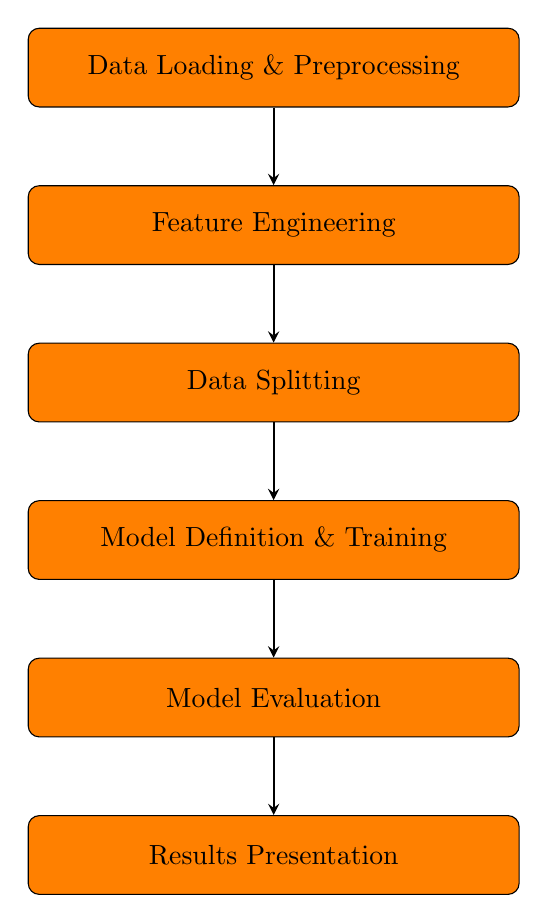
\begin{tikzpicture}
    % Define the styles for the processes and arrows
    \tikzstyle{process}=[rectangle, rounded corners, draw=black, fill=orange, text centered, text width=6cm, minimum height=1cm]
    \tikzstyle{arrow}=[thick,->,>=stealth]

    % Draw the processes
    \node[process] (data_loading) at (0, 0) {Data Loading \& Preprocessing};
    \node[process] (feature_engineering) at (0, -2) {Feature Engineering};
    \node[process] (data_splitting) at (0, -4) {Data Splitting};
    \node[process] (model_definition) at (0, -6) {Model Definition \& Training};
    \node[process] (model_evaluation) at (0, -8) {Model Evaluation};
    \node[process] (results_presentation) at (0, -10) {Results Presentation};

    % Draw the arrows between the processes
    \draw[arrow] (data_loading) -- (feature_engineering);
    \draw[arrow] (feature_engineering) -- (data_splitting);
    \draw[arrow] (data_splitting) -- (model_definition);
    \draw[arrow] (model_definition) -- (model_evaluation);
    \draw[arrow] (model_evaluation) -- (results_presentation);
\end{tikzpicture}

%     \caption{Flow diagram of the implementation process.}
%     \label{fig:flow_diagram}
% \end{figure} 

\section{\ac{lstm} Training and Testing}
\begin{itemize}
    \item Use Keras library for implementation \cite{keras}
    \item Model: LSTM layer, Dense layer with softmax activation
    \subitem Sequences are of length sliding window\_size for each entry in the dataset 
    \item sliding window size will be \(25 * 0.25 = 6.25\), so we choose 6 seconds as the sliding window size, as our dataset has \ac{wifi} timestamps for every about 2 seconds, we set window\_size = 3 \cite{EffectsSlidingWindow2022}
    \subitem Inputs are (window\_size, number\_of\_features (which are 6 + number of BSSIDs)), see \Cref{fig:lstm_architecture}
    \item Generate predictions on the test set
    \item Get class with the highest probability as prediction
    \item Get top 3 predictions for the test set and check if the target variable is in the top 3 predictions.
\end{itemize}

\begin{figure}[h!]
    \centering
    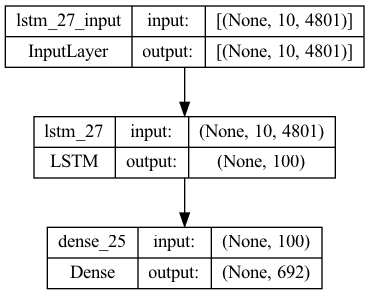
\includegraphics[scale=0.5]{images/model_plot.png}
    \caption{An example LSTM Network with Input, LSTM and Dense Layer with 4801 Features and window\_size of 10.}
    \label{fig:lstm_architecture}
\end{figure}

\section{Tuning model and hyperparameters}
\begin{itemize}
    \item try out different hyperparameters also in combination
    \subitem Number of units in the LSTM layer = \{100, 150, 200, 350, 500, 1000, 2000\}
    \subitem batch size = \{16, 32, 64\}
    \subitem window size = \{3, 5, 10, 20\}
\end{itemize}

%\noindent
